\documentclass[aip,amsmath, reprint, author-year]{revtex4-1}
\usepackage{url}
\usepackage[utf8]{inputenc}
\usepackage{hyperref}
\usepackage{graphicx} % for graphics
%\usepackage{listings} % for code listtings
%\usepackage{color}

%\setcitestyle{round, author-year}

\setcounter{page}{1}

%\bibliographystyle{aipauth4-1.bst}

\begin{document}

\begin{abstract}
An approach to generate Generalised Process Capability Data in order to populate and add functionality to a Process Capability Database.
A description of the concept of generalisation, uses and implementation.
\end{abstract}

\title{Concept of using General Process Capability Data}
\author{Andreas Bruun Okholm, s082562\\
Mathias Rask Møller, s082536 }
\affiliation{Technical University of Denmark}
 
\date{\today}
\maketitle

%Introduction

A Process Capability DataBase (PCDB) is a tool for mechanical designers to get information of what is possible to achieve in the companies production. This is done by storing and displaying statistical information about features on produced components.  
By applying Process Capability (PC) information in the design process it is possible to reduce: rework, cost, failure rate, assembly problems and increases product performance \citep{tata1999process}.

As mentioned in \citep{tata1999process, tata1999effective, raskokholm} and a number for key challenges has to be addressed to expand the use of PCDB.
\begin{itemize}
	\item Data Communication: The databases are typically not easily searchable which makes it very difficult to find the correct data and in many cases the data sought after data does not exists. Further more the data is not presented in a way which is easily understandable by mechanical designers.
	\item Fragmented Organisation: Development department are dependent on data from production. 
	\item Information Technology: Make a database which is fast, live, global, self populating, up to date and live up to the industry criteria of security and anonymity.
\end{itemize}

There has been a couple of attempts in academia to solve some of these difficulties \citep{thornton2000use, kern2003forecasting, thornton2004variation}, but there hasn't much attention on the subject since indicating there is still issues to resolve before it can be efficiently used in the industry.

In this article we present a concept of data indexing, processing and presentation which tries to make it faster and easier for the mechanical designer to efficiently use process capability data in new designs. 
The general principle is to provide an interface where the data is presented in a much more generalised than typically done in PCDB interfaces. 
The core indexing scheme is simplified, but details are retained or improved using a flexible tagging system. 
Instead of presenting the designer with statistical information, recommended specifications limits based on actual PC is shown directly. 
The specification limits is normalised in regard to the specified dimension making more use out of each dataset, minimising the risk of PC requests not returning any results. 

Combined with advances in Information Technology we hope this will help make PCDBs a viable tool in the mechanical design process. 

\section{Indexing}
PCDB data needs to be indexed to efficiently retrieve data of relevance to the current design. The data stored in a PCDBs is typically measurement sets; the statistical result of a number of measurements from a given part dimension combined with the Design Characteristics (DC). Feature, geometry, material and process is suggested by \cite{kern2003forecasting} to be the primary DC's. For each primary DC there exists a tree structure of possibilities. An example of an index using Kerns proposed design index could be "Plane", "Position", "Aluminium", "Turning" as feature, geometry, material and process respectively. 

For our index,  \emph{material} and \emph{process} should be only required DCs. This is combined with a tagging systems, where additional tags can be inputted. Common tags can be selected from tree structure. 
Tags gives more flexibility since more than one tag can be applied to one measurement set and it is possible to index for DC's that are specific to a single production method or material. 

Example: For injection moulding it would be interesting to index the material type of the mould - aluminium, steel, hardened, ... Indexing the mould iterations (T0, T1, T2) could also give valuable insights of which specification limits requires mould rework or process adjustment. Another example: To tag if the dimension measured crosses a parting line in the mould potentially showing a general increase in desired specification limits.

In casting and injection moulding which are some of the most used processes for mass produced part, feature and geometry is not necessarily important DCs. In mould making the individual geometries are manufactured in the same CAM milling machine. 
The variation in the product from the mould is most likely independent of geometry with exceptions of features that have high length to width ratios and small deep holes that are hard to manufacture. PC data for different geometries such as diameters, positions, thickness, radii are pooled together but can be marked with an exception-tag.

In a fully integrated robust design process interaction between components are reduced to as small and simple surfaces as possible. The need for indexing geometry of components should decrease.

\emph{What you measure and index is what you can analyse from.}
Since the index limits the possible conclusions, which can be mades when extracting the data. If the goal is to understand the long term process capability impact of an injection mould process it is either necessary to have measurement sets from many products at different stages of their lifespan or multiple measurements through the lifespan of a couple of products.    

\section{Processing Capability Data}

Processing the capability data consists of three steps: 

\begin{enumerate}
	\item Compute Process Capability Specification Limit (PCSL).
	\item Normalise PCSL.
	\item Interpret normalised PCSL data.
\end{enumerate}

\subsection{Process Capability Specification Limit}
The process capability indices ($C_p$ and $C_{pk}$) described by \cite{kane1986process} has been widely adopted in statistical process control, been extended and further researched for better understanding \citep{wu2009overview}. 
Instead of looking at process mean $\mu$, standard deviation $\sigma$ and specification upper and lower limits $USL$, $LSL$ using Process Capabilities Indices (PCIs) transforms these values into unit less numbers, which provides a quick overview of how a process is performing.

The PCIs ability to transform process variables of any object into unit less capability index can be reversed to calculate desirable specification limits. For en example the commonly used CPI $C_{pk}$ 
\begin{equation}
	C_{pk} = \frac{d - | \mu - m|}{3 \sigma}
\end{equation}
can be reversed
\begin{equation}
	d = 3 C_{pk} \sigma + | \mu - m|
\end{equation}
Where $d = (USL - LSL) / 2$ is half the specification limit and $m = (USL + LSL) / 2$ is the midpoint between the specification limits. Since the $d$ is the required tolerance to achieve the desired process capability index value we call this the Process Capability Specification Limit (PCSL). 

There are several commonly used PCIs each serving their purpose \citep{wu2009overview, taguchi1986introduction}
\begin{itemize}
	\item $C_a$ : Closeness of process mean to target 
	\item $C_p$ : Relative size of variation
	\item $C_{pk}$ : Amount of nonconforming (\%NC)
	\item $C_{pm}$ : Value loss (Taguchi loss function)
	\item $C_{pmk}$: Version of $C_{pm}$,  sensitive to mean shift. 
\end{itemize}

Visualising the $CPIs = 1$  shows how a process on target $C_a = 1$ allows the same variation for all PCIs see figure \ref{fig:CPI}. The line for $C_{pm}$ is in below that of $C_{pk}$ except for values of $C_a$ close to 1. 
Using $C_{pm}$ will in general be more conservative resulting in larger specification limits than $C_{pk}$. The plot shown is for a capability equal to one for higher values this effect is even more pronounced.

\begin{figure}
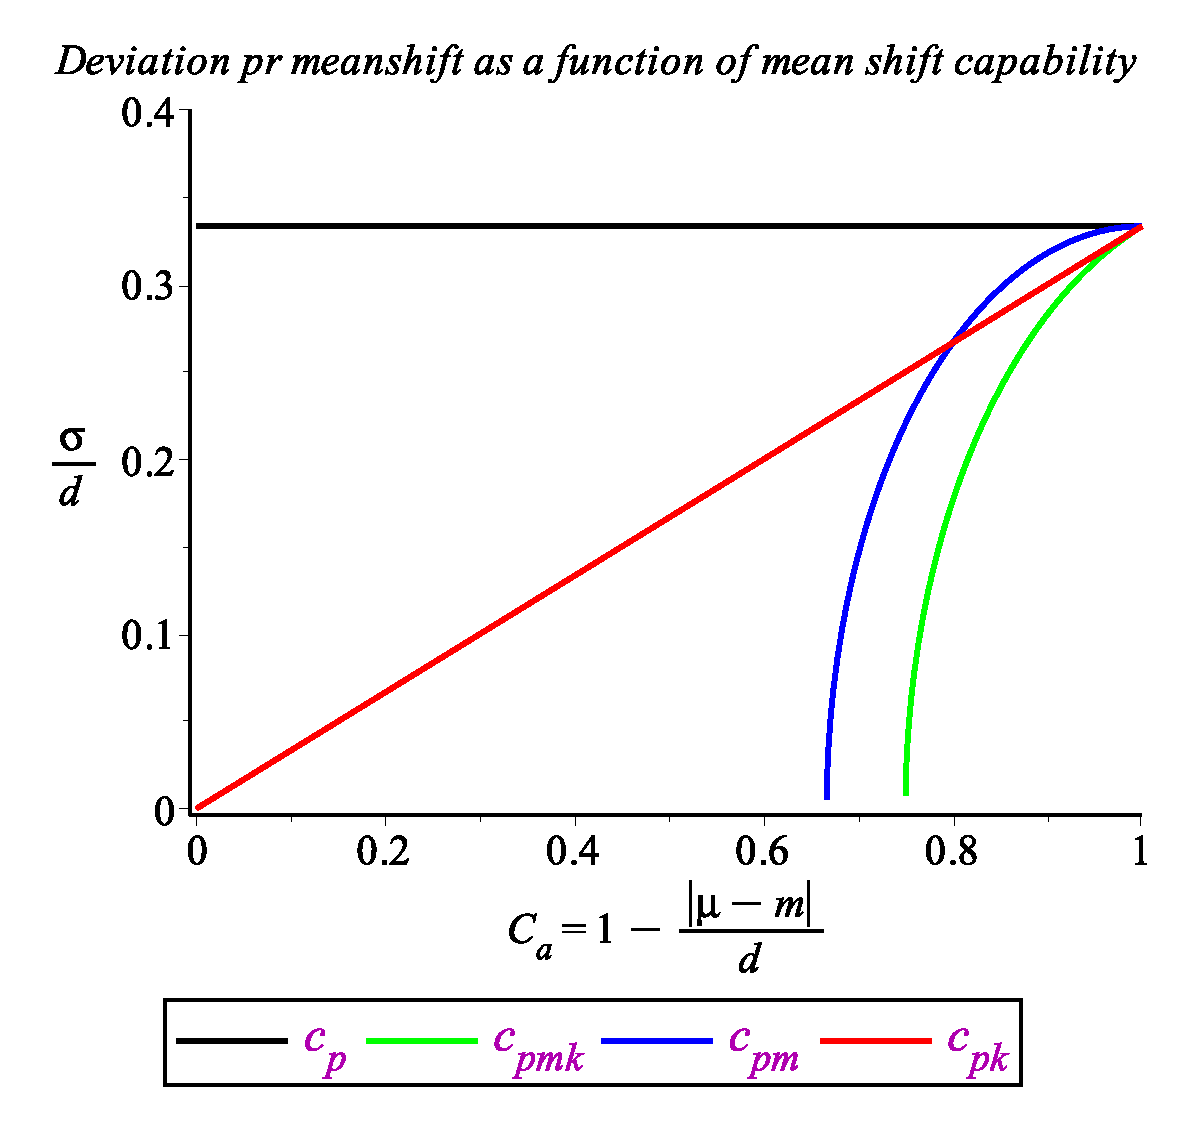
\includegraphics[width=0.45\textwidth]{graph_postscript_test.eps}
\caption{\label{fig:CPI} $C_p$ referens only to the variance of the process. $C_{pk}$ is related to the yield of the product. $C_{pm}$ takes a loss function in to account relates to a target dimension. $C_{pmk}$ takes both the yield of the product and a loss function. }
\end{figure}

For the purpose of our database we have chosen to use $C_{pk}$, since it provides the most easily understandable result - directly related to the yield of the process. The yield of a process is within $2\Phi(3C_{pk})-1 \leq \text{yield} < \Phi(3C_{pk})$ where $\Phi(\cdot)$ is the cumulative distribution function of the standard normal distribution N(0,1) \citep{boyles1991taguchi}. For typical capability levels the resulting non-conforming products in parts per million (ppm) is listed in table \ref{tab:cpl_nc}

\begin{table}
\begin{ruledtabular}
\caption{\label{tab:cpl_nc} $C_{pk}$ Non-conformities}
\begin{tabular}{llll}
  $\mathbf{C}_{pk}$	& $\sigma$ level	& $\mathbf{NC_\mathrm{max}} \mathrm{\ (ppm)}$	&  $\mathbf{NC_\mathrm{min}} \mathrm{\ (ppm)}$	\\
  1.00	& 3		& 2699.8		& 1349.9		\\
  1.33 	& 4 		& 63.3		& 31.7 		\\
  1.50 	& 4.5 	& 6.7		& 3.4		\\
  1.66	& 5		& 0.6		& 0.3		\\
  2.00	& 6		& 0.002		& 0.001		\\
\end{tabular}%
\end{ruledtabular}
\end{table}

The optimal process capability index values depends on the application, however there exists a practice in quality control called six sigma $(6 \sigma)$, which advocates the use of six sigma ($C_{pk} = 2$) for short term process capability will generally improve manufacturing quality and profits \cite{koch2004design}. 
It's assumed that the process drifts over time up to $1.5 \sigma$ (effectively resulting in a sigma level of 4.5), which still results in an acceptable 3.4 ppm defects. 
Depending wether the data inputed into the PCDB are mostly from newly setup processes or long term samples the $C_{pk}$ should be varied from 2.0 to 1.5 to achieve six sigma for the process. 
We propose to use a value of $C_{pk} = 1.66$, which would result in six sigma levels of performance if the inputed datasets are a mixture of long term and short term measurements. 
Alternatively it would be possible to set an acceptable $C_{pk}$ value when inputing each measurement set depending weather the measurement set reflects the short or long term capability. 

We have focused on $C_{pk}$ through most of this section.
In situations where the desired tolerances directly influence product performance, for instance in lens optics construction, using the more abstract $C_{pm}$ might make more sense. 

\subsection{Normalization}

The calculated Process Capability Specification Limits (PCSL) are normalised so it can be used to predict PCSLs for any dimension within the limit of the normalisation algorithm. 
This reduces the required amount of data in the database before it's useful for mechanical design since it is possible to use PC information from components of different sizes.

There exists industrial standards used for manufacturing which describe the 'normal' relationships between linear dimensions and tolerances. We have analysed the most commonly used standards for general tolerances: American \citeauthor{american1978preferred}, European ISO 286-2 (1993 ) and the German standard \citeauthor{DIN7168}.
and the 

   and have slight difference but all present a nonlinear curve. For the same level for precision the tolerance of big dimensions is smaller relative to size than for component of a small dimension.
For general linear tolerances as described in American ANSI B4-2 (1978) and the German DIN7168 (1991) have slight difference but all present a nonlinear curve. For the same level for precision the tolerance of big dimensions is smaller relative to size than for component of a small dimension.

The german standard \citeauthor{DIN16901} and the French \citeauthor{NFT58000} are standards that specifically relates to moulded plastic parts. These standards present an almost linear function. The difference can be a result of the creep in moulded plastic that is a percentage of volume and not a function of dimension.

In figure ~\ref{fig:tolstd} both the standards for general and moulded plastic specific linear tolerances are shown.

\begin{figure}
\includegraphics[width=0.5\textwidth]{Tolerance_standards.pdf}
\caption{\label{fig:tolstd} The danish standard DS812 (POM 120) and the French NFT58000 (normal) are standards specifically for moulded plastic components. They are almost linear for sizes above 10 mm The American ANSI B4-2 (gr. 13) and the german DIN7168 (medium) describes the linear tolerances dimension relation. The tolerance is smaller for }
\end{figure}

The descriptions of the standards presents the data as tables for tolerances in dimension intervals. This poses a problem when trying classify the specific tolerance dimension to a precision level.
In a note for ANSI B4-2  and later mentioned in ISO 286:1993 a continuous function is described for IT-grades between IT6 to IT16 for dimensions from 2 mm to 500 mm. This function is not included in newer versions of ISO 286.

\begin{align}
	T =& 10^{0.2 (ITG -1)} \cdot i \\
	i =& 0.45 \sqrt[3]{D} + 10^{-3} \, D 
\end{align}

Where $i$ is standard tolerance factor, $D$ is the nominal mean dimension $D = \sqrt{D_{\textrm{min}} D_\textrm{max}}$ in $[mm]$ and $T = 2 d$ is the tolerance width in $[\mu m]$. 

In the generalised PCDB the data is normalised using said function because ISO 286 is general practice in the industry. 
Further work on improving the normalisation feature is possible, when more PCDB data is available and it's possible to do an fit to the actual data for the different processes.

\subsection{Analyze normalized data}

The analysis is done to present the user with a useful information through graphics based on data of  a subset of DC's selected by the user. 

To help the user determine which tolerance to use, a accumulated frequency plot of the normalised PCSL is proposed. 
This gives an overview of the current process process capability assuming it has not changed since the data has been recorded. 
The plot shows the probability, if production capability were randomly selected, to produced the selected part at a specified $C_{pk}$ and tolerance, see figure \ref{fig:acumfreq}. 
A normal distribution is fitted to the data to shown a continuous function.
% Confidence intervals for the distribution is calculated to to show the validity of the estimate.

The 



A tolerance of low probability can have impact to the price of production since it either: Risks the larger change for need of rework to hit the target $C_{pk}$. Requires more precise machines than what is used for the sample.

\begin{figure}
\includegraphics{Acum_freqIT.pdf}
\caption{\label{fig:acumfreq} Accumulated frequency IT grade distribution, $C_{pk} =1.66$. 
20 sample set each of a between 3 and 219 samples. Actual data from \cite{thornton2000use}. }
\end{figure}

By selecting more than one subset of DC's for comparison it is possible to get a view of the individual subset. In figure \ref{fig:acumfreqF3} PC data from two machines is shown respectively. It is possible to see that the machine marked '1031' performs better than '1032' it is therefore better.

\begin{figure}
\includegraphics{Acum_freqF3.pdf}
\caption{\label{fig:acumfreqF3} Data from 2 subsets for DC's. Measurement sets from machine nr. 1031 and 1032 respecfully. Accumulated frequency IT grade distribution, $C_{pk} =1.66$. Actual data from \cite{thornton2000use}. }
\end{figure}

Further consideration are done in order display the information in a more comprehensible way.
\begin{itemize}
\item The tolerance can be shown in $[mm]$ for a user selected dimension.
\item Include popup interactivity allowing the user to see specifics of each data point.
\item Show the confidence limits for the estimated distribution.
\end{itemize}

\section{Statistical Validity}

\emph{What you measure is what you can analyse.}  
To determine the sample size needed to represent a population of 


Each product in the sample set, produces a measurement. From the sample set is a  measurement set created. 

Confidence intervals - sample size of each measurement set.

Measurement sets are assumed to fit a normal distribution.


\begin{figure}
\includegraphics{stats_std_confidence.pdf}
\caption{\label{fig:std_uncertainty}The uncertainty of the standard deviation estimate is reduced as the number of samples is increased. The increase in accuracy gained per additional decreases with more samples. From the graph we have chosen 12 to be the optimal point for general process capability use.}
\end{figure}

\begin{figure}
\includegraphics{CLW90_surf.pdf}
\caption{\label{fig:cl_surf}The uncertainty of the standard deviation estimate is reduced as the number of samples is increased. The increase ind accuracy gained per additional decreases with more samples. From the graph we have chosen 12 to be the optimal point for general process capability use.}
\end{figure}

\begin{figure}
\includegraphics{CLW90_lines.pdf}
\caption{\label{fig:cl_line}The uncertainty of the standard deviation estimate is reduced as the number of samples is increased. The increase in accuracy gained per additional decreases with more samples. From the graph we have chosen 12 to be the optimal point for general process capability use.}
\end{figure}

Number of measurement sets to predict process capability.  


show current production capability in terms of it-grade

\section{Using the general process capability data}
apply tolerance, By looking at normalised data of the variance of products of the same material and process, it is possible to find a suitable tolerance
improvement per rework
material selection


\section{Discussion}

Using todays technology, generalisation of PC data upon request from the user I feasible. A proposed technical setup is described in \cite{OkholmRask}.

Initiating PCG is a tough process. 
The reward for doing robust design engineering is long reach
The reward for using PCDB or robust design in general to make changes in early design is a long term and might only benefit the company and not feedback to the designers compared the reward for the hero in production solving the expensive errors in design.

Implementing GPC requires a change
	economical barrier
		big company
			incement from quality department
			gain: 	knowledge of own PC
					high precision data
					Extensive knowledge on causes and problem
			Loss:
		cross companies
			diverse data
			gain:		Alot of data
					knowledge of processes and material outside your field
					knowledge of possible to achieve in industry
					Index storing of own data and partially analysed
			loss:		Industry espionage concerns
					loss of information due to anonymity

proto running at a university, unbiased.


\section*{References}
\bibliography{../PCDBmasterBibliography/PCDB_Master_bib.bib}

\end{document}